% !TeX document-id = {817cd221-9a0f-4126-a2d0-e6c949256717}
% !TeX TXS-program:compile = txs:///pdflatex/[--shell-escape]
% % !TEX TS-program = xelatex
% !TEX encoding = UTF-8 Unicode

% Spring 2020 - Summer 2020 - Fall 2020
% Tristan Hill, May 07, 2020 - June 12, 2020 - July 08, 2020 - Novemeber 02, 2020
% Module 11 - Probability and Statistics
% Topic 1 - Histograms and Probability Density Functions

\documentclass[fleqn]{beamer} % for presentation (has nav buttons at bottom)

\usepackage{../../measurements_lectures}
\usepackage{listings}

% \usepackage{minted}
% \setminted[text]{
% 	escapeinside=||, 
% 	frame=single,
% 	framesep=2mm,
% 	baselinestretch=1.2,
% 	bgcolor=mygray
% }
% \setminted[cpp]{
% 	escapeinside=||, 
% 	frame=single,
% 	framesep=2mm,
% 	baselinestretch=1.2,
% 	bgcolor=mygray
% }

\author{ME3023 - Measurements in Mechanical Systems} % original formatting from Mike Renfro, September 21, 2004

\newcommand{\MNUM}{12\hspace{2mm}} % Module number
\newcommand{\TNUM}{1\hspace{2mm}} % Topic number 
\newcommand{\moduletitle}{Probabilities and Statistics}
\newcommand{\topictitle}{Histograms and Probability Density Functions} 

\newcommand{\sectiontitleI}{A Population of Data}
\newcommand{\sectiontitleII}{Randomly Distributed Data}
\newcommand{\sectiontitleIII}{Frequency Histogram}
\newcommand{\sectiontitleIV}{Probability Density Function}

% custom box
\newsavebox{\mybox}

\title{Lecture Module - \moduletitle}

\date{Mechanical Engineering\vspc Tennessee Technological University}

\begin{document}
	
	\lstset{language=MATLAB,basicstyle=\ttfamily\small,showstringspaces=false}
	
	\frame{\titlepage \center\begin{framed}\Large \textbf{Topic \TNUM - \topictitle}\end{framed} \vspace{5mm}}

% Section 0: Outline
\frame{
\large \textbf{Topic \TNUM - \topictitle} \vspace{3mm}\\

\begin{itemize}

	\item \sectiontitleI    \vspc % Section I
	\item \sectiontitleII 	\vspc % Section II
	\item \sectiontitleIII 	\vspc %Section III
	\item \sectiontitleIV 	\vspc %Section IV

\end{itemize}

}

\section{\sectiontitleI}	
	% Section I - Frame I
	\begin{frame}[label=sectionI] \small
		\frametitle{\sectiontitleI}    
		
		Consider a manufacturer that makes 100000 of ball bearings in a set. \vspace{3mm}
		
		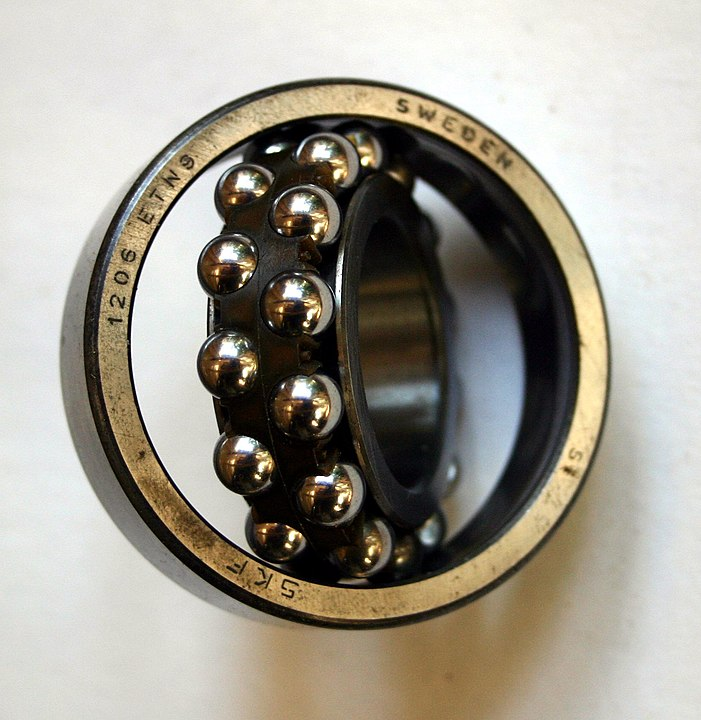
\includegraphics[scale=.1]{bearing_fig1.jpg} \hspace{10mm}
		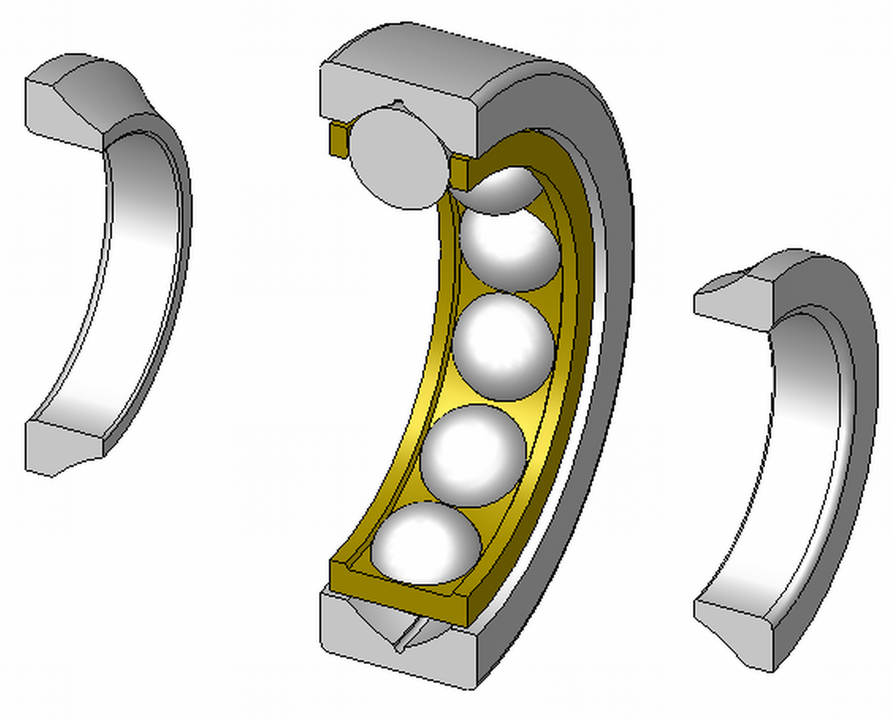
\includegraphics[scale=.1]{bearing_fig2.png} \hspace{10mm}
		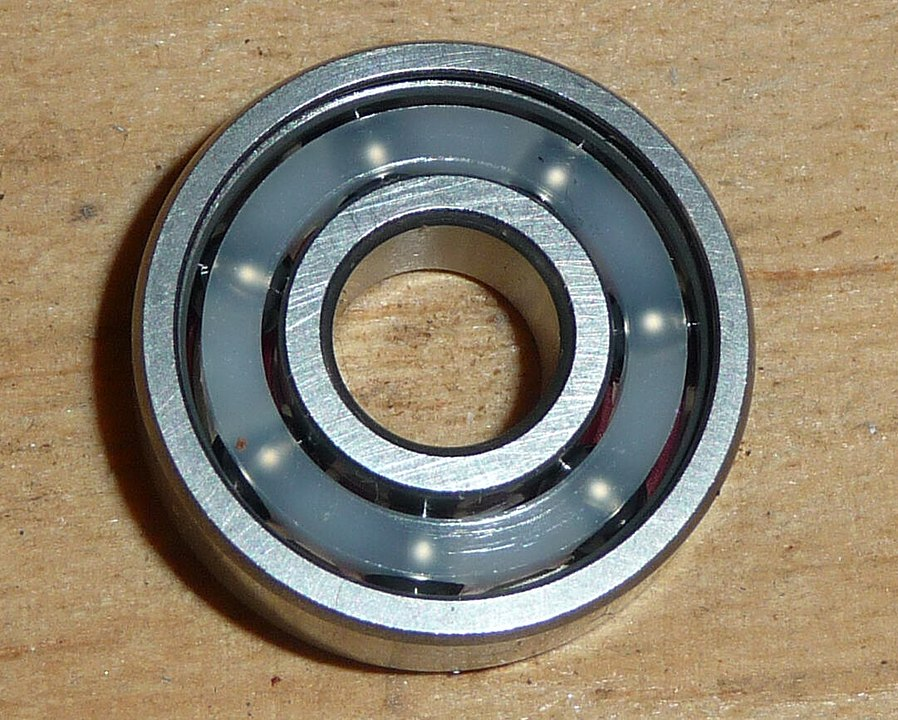
\includegraphics[scale=.1]{bearing_fig3.jpeg}
		\begin{itemize}		
			\item How does the manufacturer ensure the quality of the product?
			\item How the does the seller communicate this to the buyer?
			\item How does the engineer use this information? 
		\end{itemize}
		
		{\tiny Images: \href{https://en.wikipedia.org/wiki/Ball_bearing}{Wikipedia} }

	\end{frame}
	
	% Section I - Frame II
	\begin{frame} \small
		\frametitle{\sectiontitleI}    
		
		%\textbf{What do we mean by a population of data?}
		 
		 The data set, or population, is generated by taking measurements of individuals chosen randomly from the entire population. \\ 
		 
		 {\bf \RD Sampling} refers to repeated measurements of the {\bf \PR measured variable} under fixed operating condition.	\\
		 
		 \[ X = \{ x_1,x_2,x_3, ... , x_i , ... , x_{n-1}, x_{n} \}  \]

	\end{frame}

\section{\sectiontitleII}	
	% Section II - Frame I
	\begin{frame}[label=sectionII] \small
		\frametitle{\sectiontitleII}    
		
				
		Our discussion will assume that the values in the data set are {\bf \PN randomly distributed } about a mean value. It is important to consider what this means.
		

	\end{frame}


\section{\sectiontitleIII}	
	% Section III - Frame I
	\begin{frame}[label=sectionIII] \small
		\frametitle{\sectiontitleIII}    

		"A {\GR histogram} is an accurate representation of the distribution of numer-
ical data. It is an estimate of the probability distribution of a continuous
variable (CORAL ) and was first introduced by Karl Pearson.[1] It differs
from a bar graph, in the sense that a bar graph relates two variables, but a
histogram relates only one." - Wikipedia

	\end{frame}
	
	% Section III - Frame II
	\begin{frame}[containsverbatim] \small
		\frametitle{\sectiontitleIII}    

%        \begin{minted}{text} 
%sudo apt install ros-|\rosdistro|-turtlebot3
%	\end{minted}
Consider sampling the 0.5 inch diameter ball bearings.
%		\begin{minted}[fontsize=\tiny]{text}
%\scalebox{1}{
%\begin{verbatim}
\lstset{basicstyle=\scriptsize}


\begin{lstlisting}
0.5016 0.4991 0.4981 0.5003 0.4988 0.5007 0.4994 0.5000 0.4999 0.4999 0.4988  
0.4997 0.4991 0.4986 0.5000 0.5018 0.4996 0.5010 0.4991 0.5011 0.5006 0.5006  
0.5014 0.5001 0.4997 0.4994 0.5001 0.5009 0.5009 0.4992 0.4983 0.5004 0.5005 
0.5004 0.4992 0.5009 0.5003 0.5018 0.5004 0.4996 0.5014 0.4992 0.4986 0.5002 
0.4986 0.4992 0.5003 0.5002 0.4999 0.4998 0.5013 0.5009 0.5003 0.4986 0.4991
0.5030 0.4995 0.5012 0.5005 0.4992 0.4995 0.5005 0.5000 0.5005 0.4993 0.4987 
0.4992 0.5018 0.4976 0.5003 0.4991 0.5007 0.5002 0.4980 0.5004 0.5000 0.4997 
0.5002 0.5004 0.4980 0.5011 0.5003 0.5013 0.5000 0.5001 0.5003 0.5000 0.5013  
0.5004 0.4988 0.5003 0.4999 0.5004 0.4996 0.4999 0.5000 0.4993 0.5003 0.4996  
0.4992 0.5008 0.4997 0.5004 0.4998 0.4998 0.5006 0.5002 0.5010 0.5014 0.5019
0.5008 0.4997 0.5002 0.4993 0.4995 0.5007 0.4986 0.5009 0.4999 0.5002 0.5010  
0.4996 0.4993 0.4982 0.4994 0.4993 0.4995 0.5002 0.5004 0.4999 0.5005 0.4993 
\end{lstlisting}
%\end{verbatim}
%}
%		\end{minted}
		
		{\tiny Data: Generated in MATLAB, see probabilty\_statistics\_topic1.m }

	\end{frame}

% Section III - Frame III
	\begin{frame}[containsverbatim] \scriptsize
		\frametitle{\sectiontitleIII}    

		\textbf{Activity:} Complete this activity as an individual.

			\begin{enumerate}
				\item Sample 20 values from the population on the previous slide. It will help to write them down in a collumn. 
				\item Choose an appropriate bin size and limits for a histogram to represent the data. The goal is to show the central tendancy and distribution of the sampled data.
				\item Create a histogram using the sampled data. Label the axis and use gridlines.	\vspace{5mm}\\
			\end{enumerate}

		\textbf{Submission:} Upload an image of your histogram and any supporting calculations to the folder {\it Concept Example: Sketch Histogram}	

	\end{frame}


	% Section III - Frame III
	\begin{frame} \small
		\frametitle{\sectiontitleIII}    

	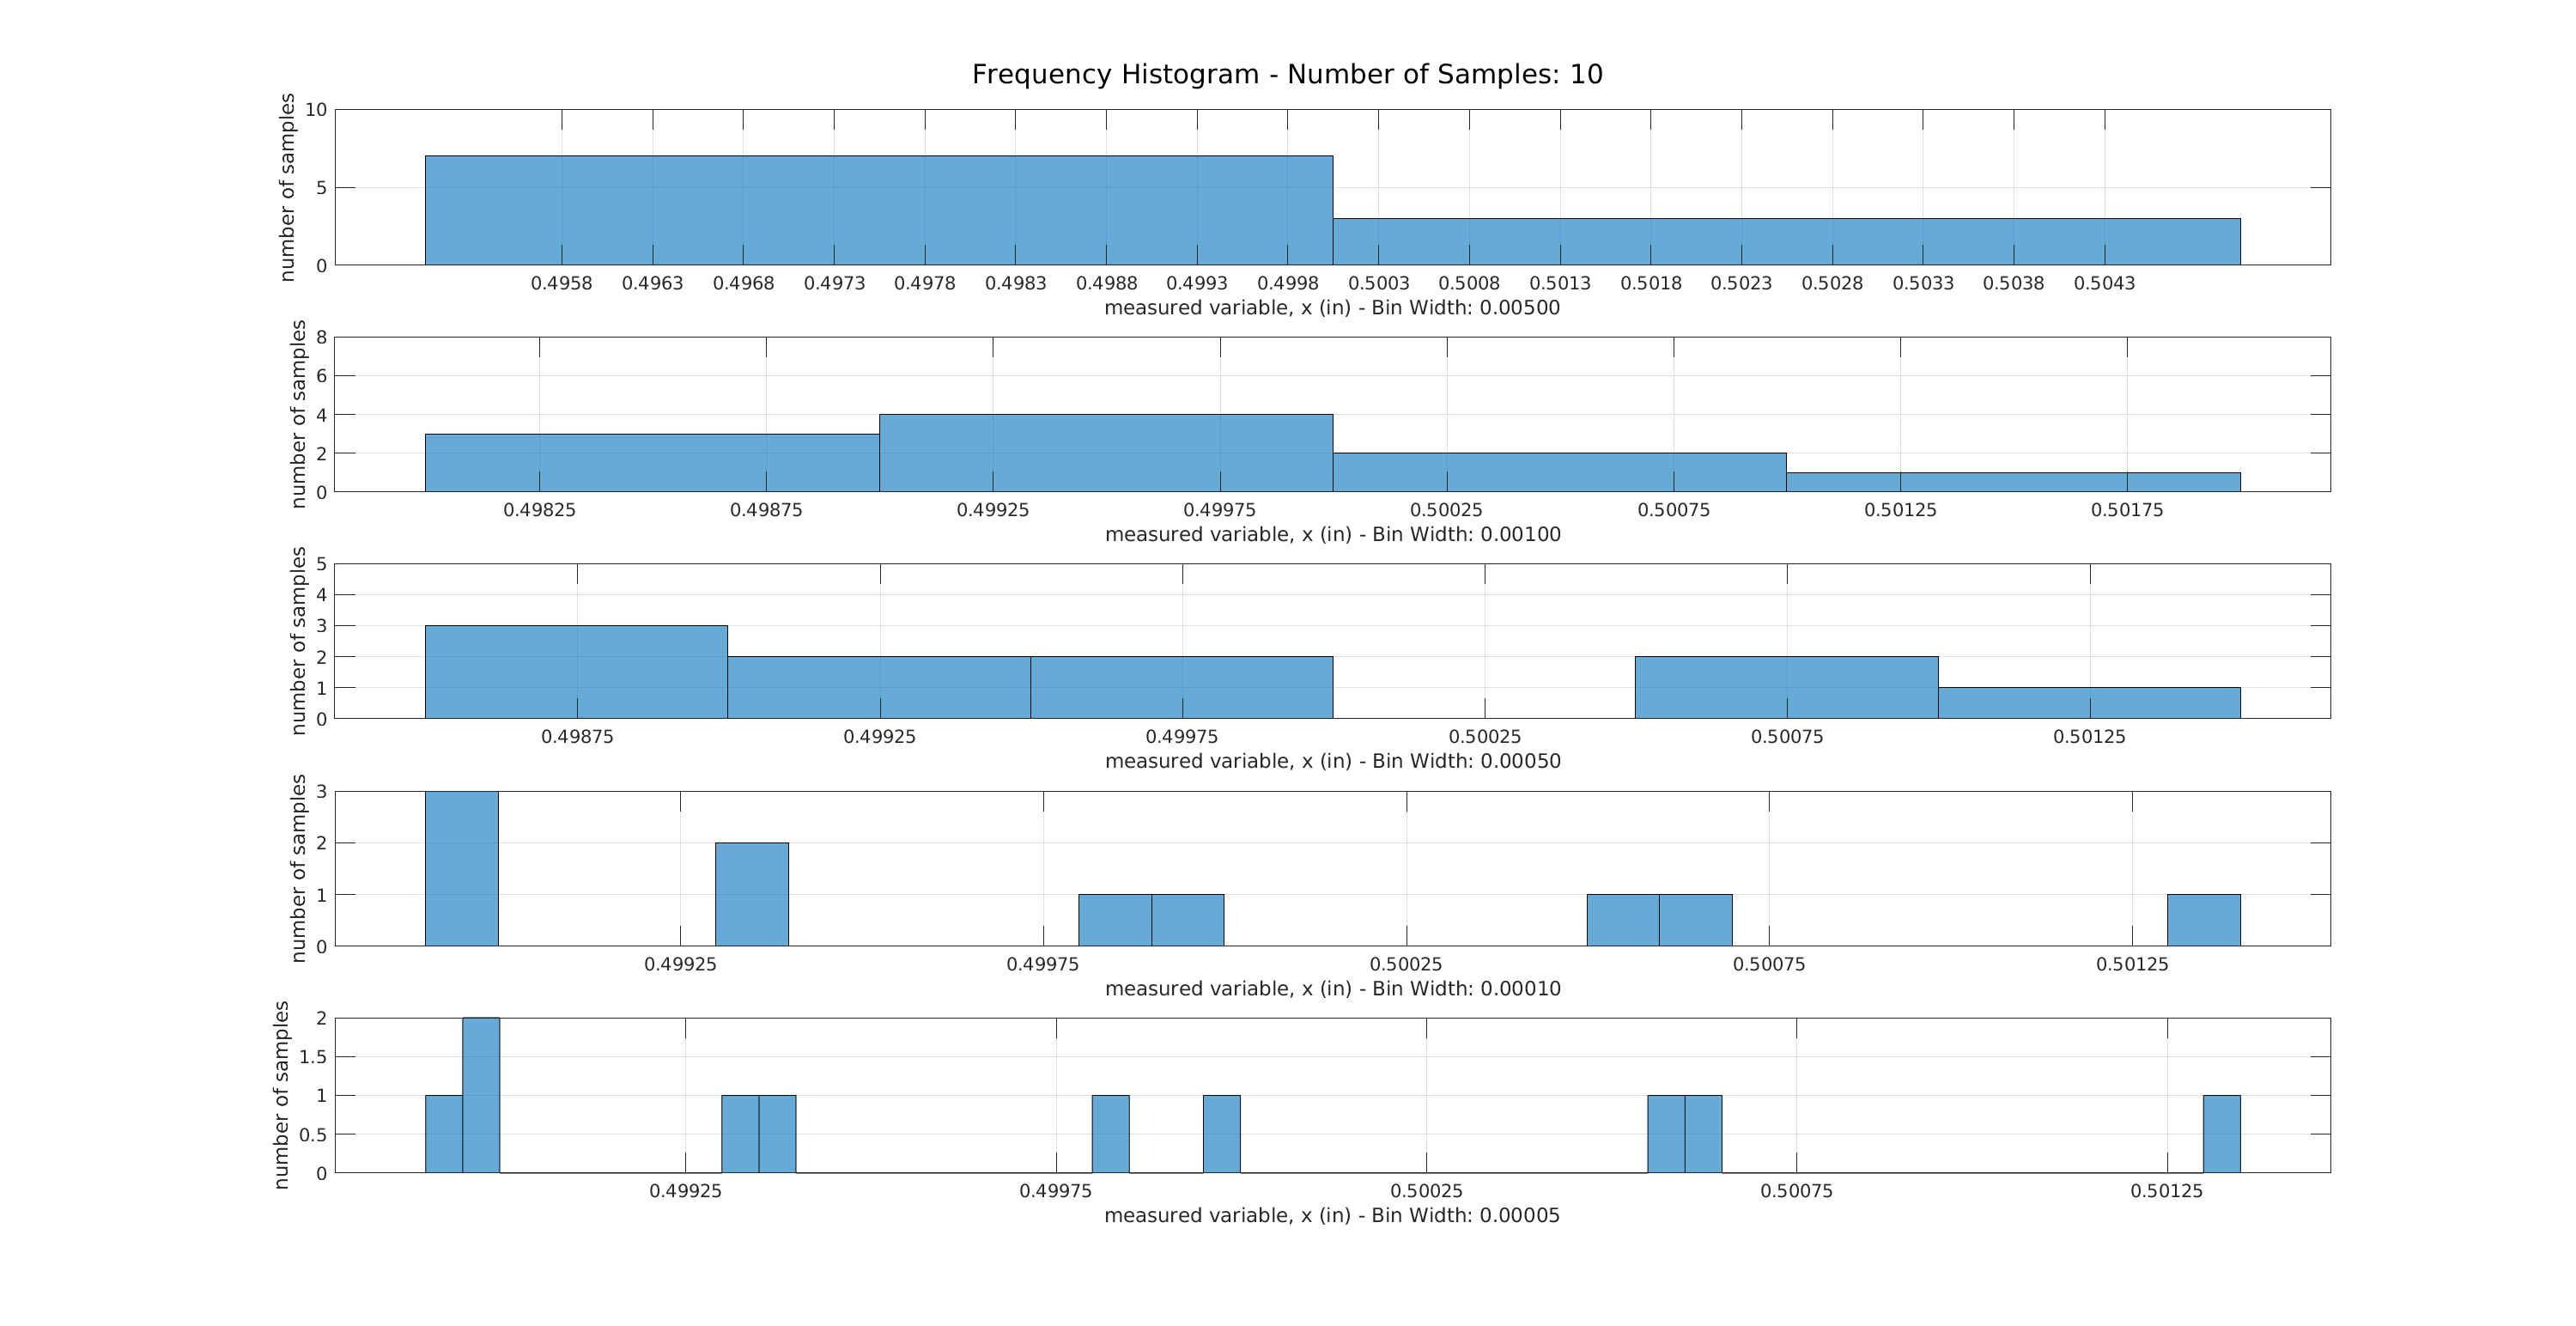
\includegraphics[scale=.25]{topic2_histogram_fig1}


	\end{frame}
	
	% Section III - Frame IV
	\begin{frame} \small
		\frametitle{\sectiontitleIII}    

	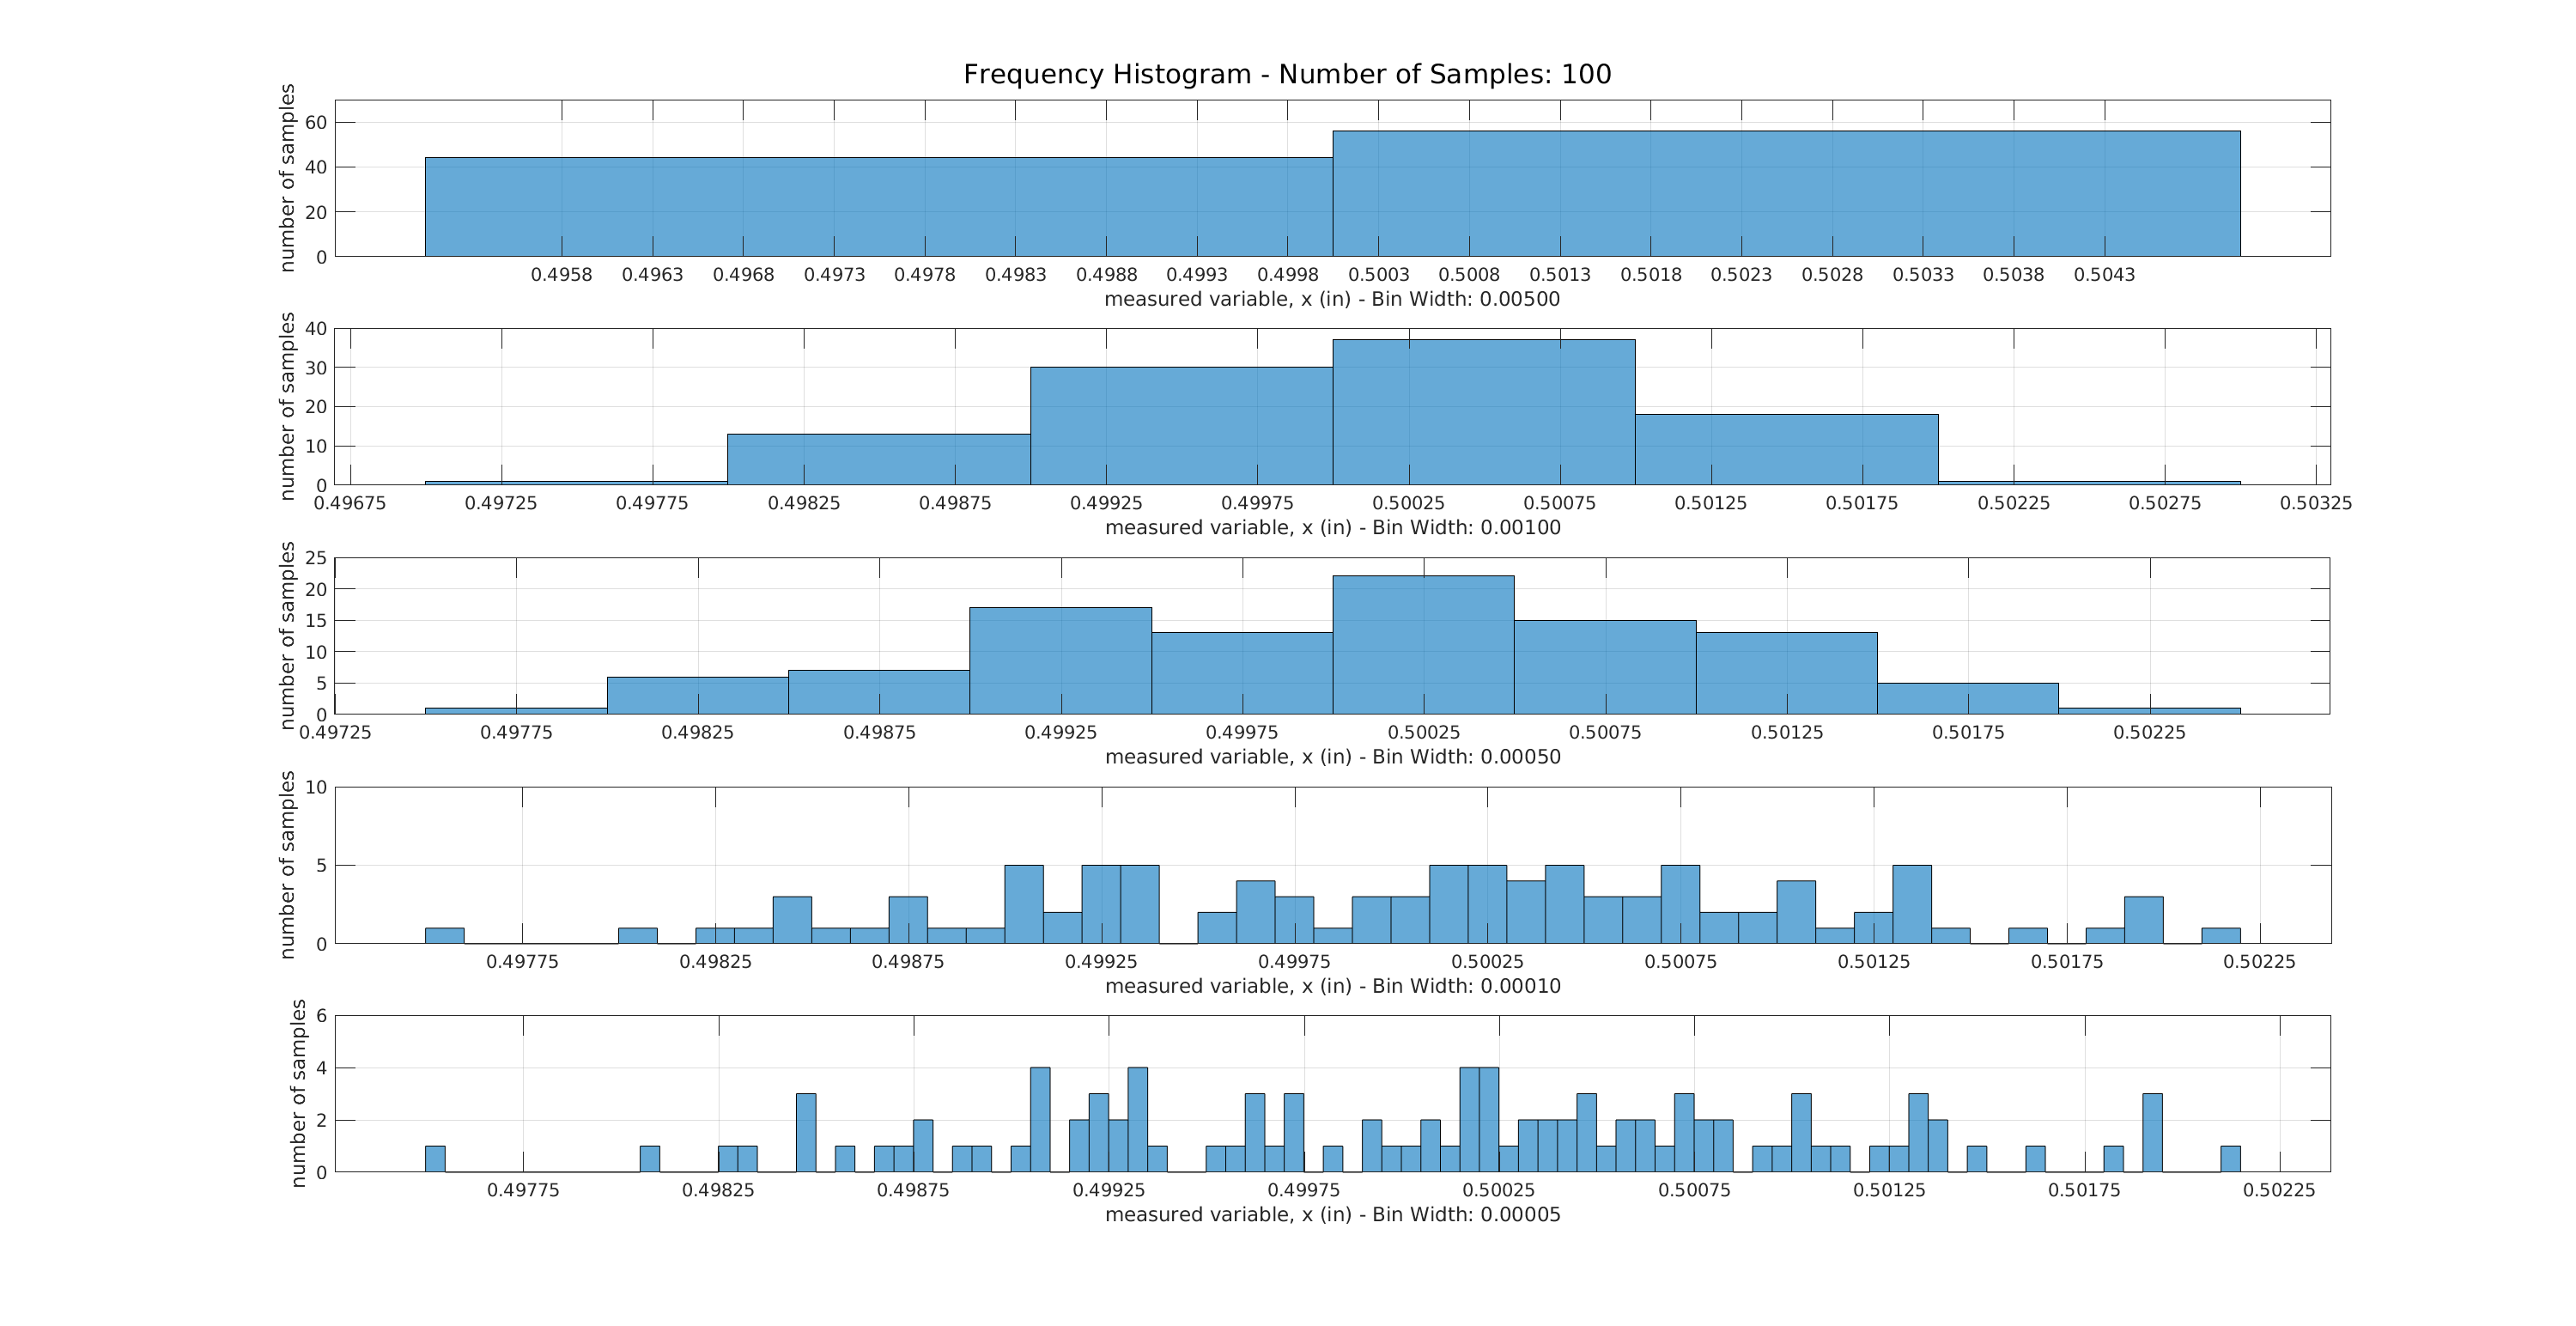
\includegraphics[scale=.25]{topic2_histogram_fig2}


	\end{frame}
	
	% Section III - Frame IV
	\begin{frame} \small
		\frametitle{\sectiontitleIII}    

	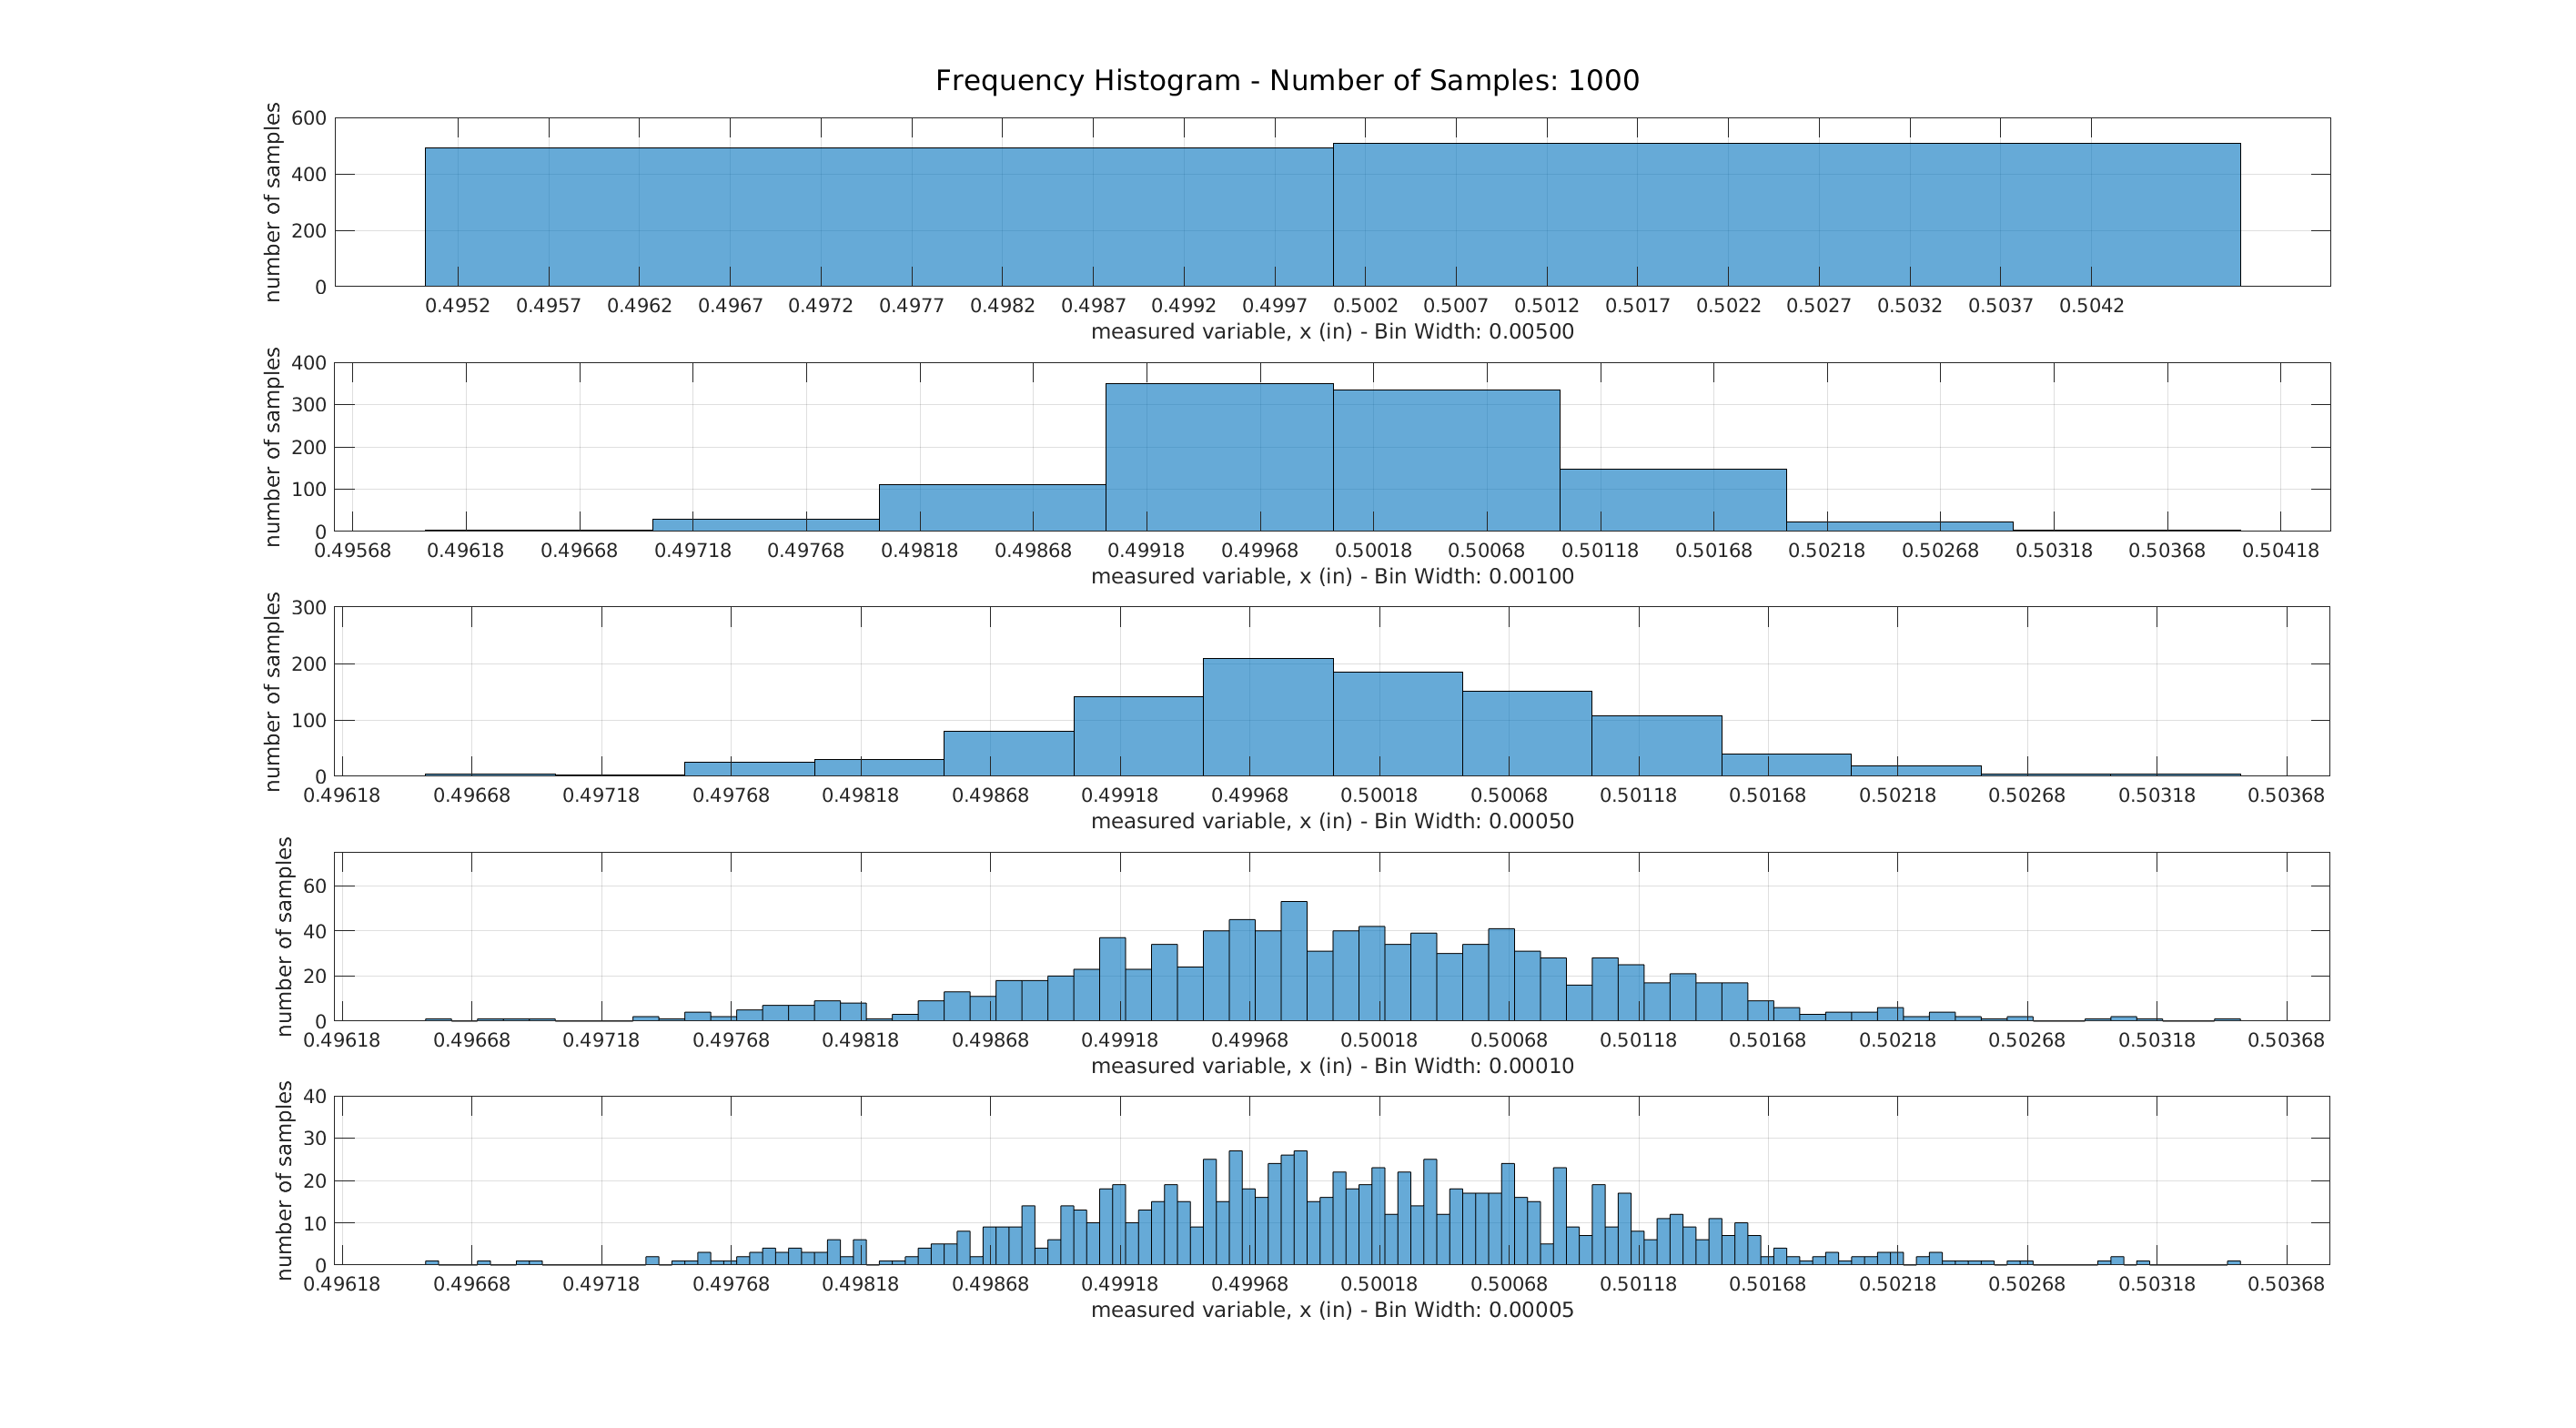
\includegraphics[scale=.25]{topic2_histogram_fig3}


	\end{frame}
	
	% Section III - Frame IV
	\begin{frame} \small
		\frametitle{\sectiontitleIII}    

	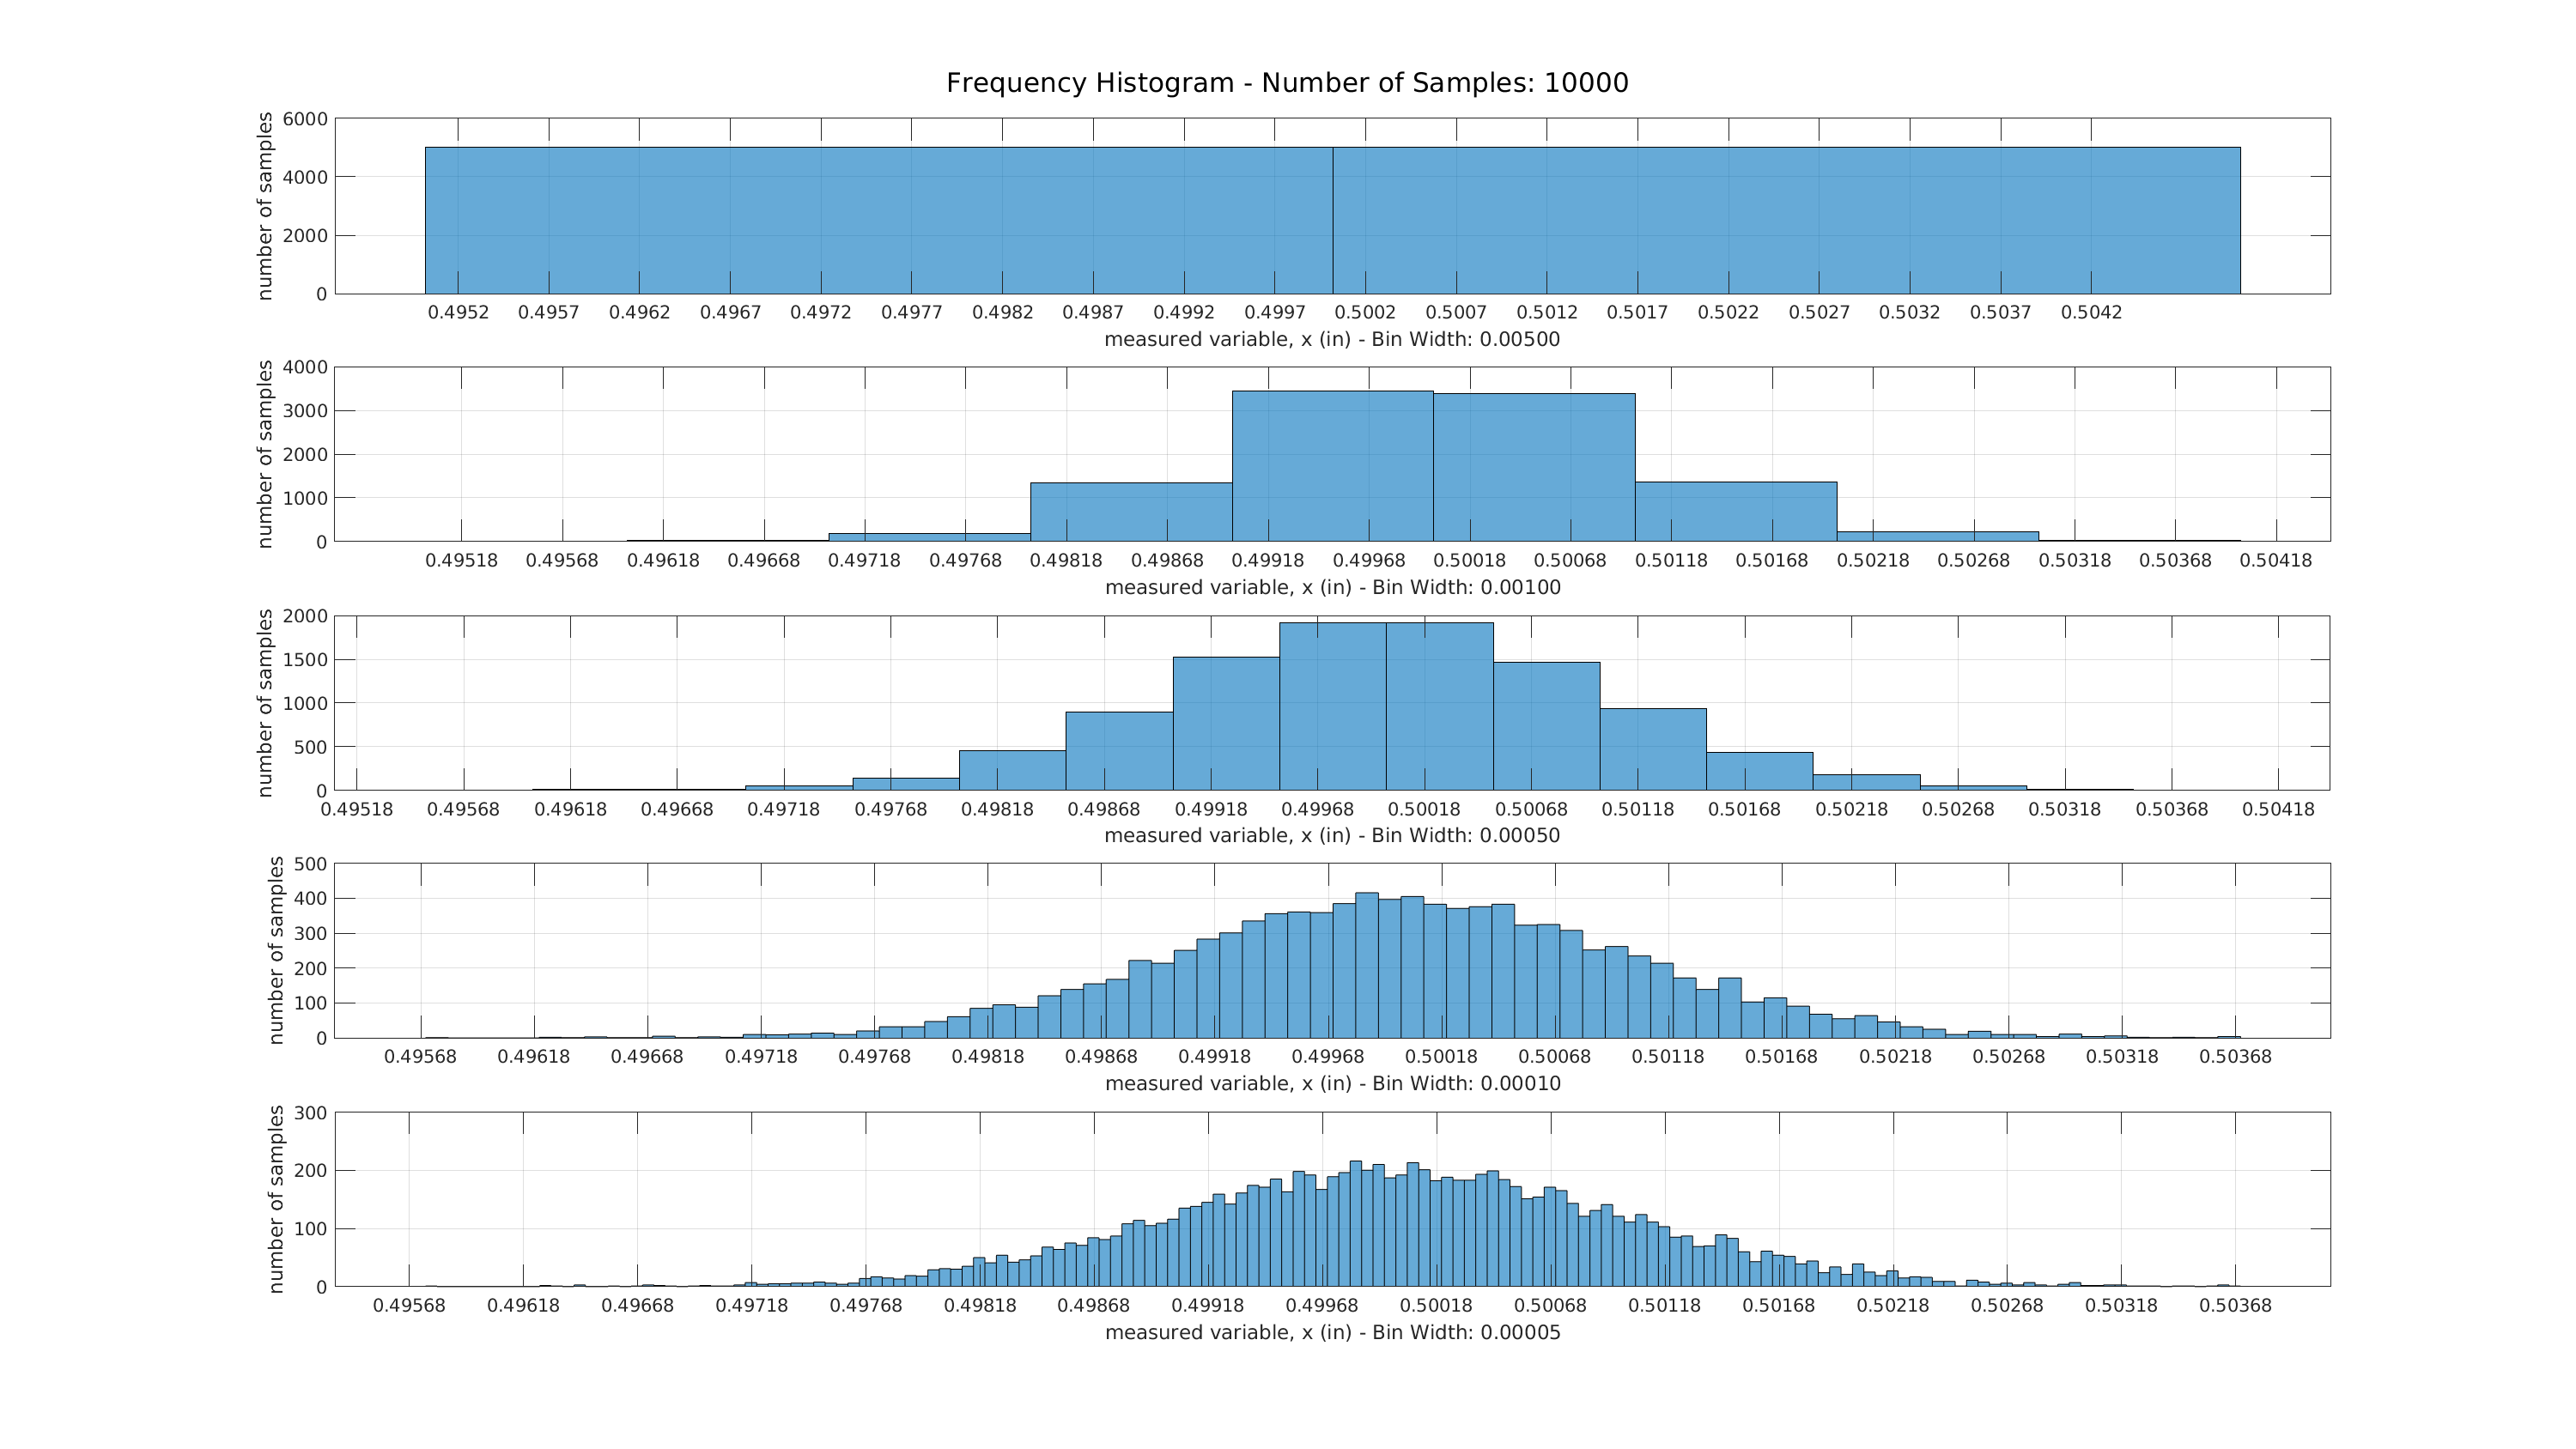
\includegraphics[scale=.25]{topic2_histogram_fig4}


	\end{frame}


\section{\sectiontitleIV}	
	% Section IV - Frame I
	\begin{frame}[label=sectionIV] \small
		\frametitle{\sectiontitleIV}    

"... a {\BL probability density function (PDF)}, or density of a continuous ran-
dom variable, is a function whose value at any given sample (or point) in
the sample space (the set of possible values taken by the random variable)
can be interpreted as providing a relative likelihood that the value of the
random variable would equal that sample ... the PDF is used to specify
the probability of the random variable falling within a particular range of
values, as opposed to taking on any one value. This probability is given
by the integral of this variable’s PDF over that range—that is, it is given
by the area under the density function but above the horizontal axis and
between the lowest and greatest values of the range ..." - wikipedia

	\end{frame}
	
	% Section IV - Frame II
	\begin{frame}[label=sectionIV] \small
		\frametitle{\sectiontitleIV}    

			\begin{itemize}
			\item  The frequency with which the measured variable assumes a particular value or interval of values is described by its {\bf \BL probability density function}. \\

            \item  If a {\bf \PR central tendency} exists we should be able to see this in the {\bf \BL probability density function}. \\
                               
            \item  As binsize of the {\bf \GR histogram} of the data set goes to zero this becomes the {\bf \BL probability density function}. \\ 
                                
		\end{itemize}

	\end{frame}

	% Section IV - Frame III
	\begin{frame}[label=sectionIV] \small
		\frametitle{\sectiontitleIV}    
Now, lets's do an example.

	\end{frame}



\end{document}

%\begin{itemize}
%
%
%	\item \textbf{ \LARGE 4.1 -  Introduction  } \\\\
%	
%		\textbf{\Large Who has taken a statistics class before? In college? In high-school?} \\\\
%		 
%		\textbf{\Large What does probability and statistics have to do with mechanical engineering?} \\\\
%		
%		
%		 \textbf{\Large For a given set of measurements we want to quantify...}
%		
%		\begin{itemize}
%			\item \textbf{\Large a representative value that characterizes the average of the measured data set} \vspace{5mm}
%			\item \textbf{\Large a representative value that provides a measure of the variation in the data set} \vspace{5mm}
%			\item \textbf{\Large how well the average of the measured data set represents the average of the entire population}  \vspace{5mm}
%		\end{itemize}
%		
%		\newpage
%		
%	\item \textbf{ \Large 4.2 -  Statistical Measurement Theory  } \\\\
%	\begin{itemize}
%		\item \textbf{ \Large Where does the measured data set come from?  } \\\\
%		\item \textbf{ \Large {\bf \R Sampling} refers to repeated measurements of the \\ {\bf \PR measured variable} under fixed operating conditions. } \\\\
%		\item \textbf{ \Large We will ignore {\bf \B systematic error} for this discussion, is this valid? } \\\\
%		
%		\item \textbf{ \Large Instead we will focus on {\bf \G random error}, its affects and how to quantify it. } \\\\
%		
%		\item \textbf{ \Large Question: If the error is really {\bf \G random error}, what is the average error? } \\\\
%		
%		
%		\newpage
%		\item \textbf{ \Large We want to estimate the {\bf \B true mean}, $x'$ from repeated measurement of $x$.} \\\\ 
%		
%		\item \textbf{ \Large The {\bf \B true mean}, $x'$ is the average of all possible values of $x$. We never actually get this!} \\\\ 
%		
%		\item \textbf{ \Large Through sampling we can find $\bar{x}$, the {\bf \G sample mean} value of $x$. We do get this!} \\\\ 
%		
%		\item \textbf{ \Large As our sample size increases, $\bar{x}$ approaches $x'$. } \\\\ 
%		
%		\scalebox{3}{$x'=\bar{x}\pm u_{\bar{x}}$}\\\\
%		
%		\item \textbf{ \Large Therefore, the sample mean $\bar{x}$ is the most probable estimate of the true mean $x'$. } \\\\ 
%		
%		\item \textbf{ \Large $\pm u_{\bar{x}}$ is the {\bf \PR uncertainty interval} in that estimate at some probability level, P\%. } \\\\ 
%	
%	         \item \textbf{ \Large The  {\bf \PR uncertainty interval} is the range about $\bar{x}$ that you would expect $x'$ to lie. } \\\\ 
%	         
%	\end{itemize}
%	%	\includegraphics[scale=0.7]{chapter3_figure_3_1.png} \vspace{20mm}\\
%		
%	%	\includegraphics[scale=1]{chapter3_figure_3_2.png}
%		
%		\newpage
%		\item \textbf{ \LARGE Histogram } \\\\ 
%			\textbf{ \large "A histogram is an accurate representation of the distribution of numerical data. It is an estimate of the probability distribution of a continuous variable (CORAL ) and was first introduced by Karl Pearson.[1] It differs from a bar graph, in the sense that a bar graph relates two variables, but a histogram relates only one. " - Wikipedia }\\
%		\item \textbf{ \LARGE Probability Density Functions  } \\\\ 
%\textbf{ \large "... a probability density function (PDF), or density of a continuous random variable, is a function whose value at any given sample (or point) in the sample space (the set of possible values taken by the random variable) can be interpreted as providing a relative likelihood that the value of the random variable would equal that sample ... the PDF is used to specify the probability of the random variable falling within a particular range of values, as opposed to taking on any one value. This probability is given by the integral of this variable's PDF over that range—that is, it is given by the area under the density function but above the horizontal axis and between the lowest and greatest values of the range ..." - wikipedia }\\
%		\begin{itemize}
%			\item \textbf{ \large The frequency with which the measured variable assumes a particular value or interval of values is described by its {\bf \B probability density function}.} \\
%
%                               \item \textbf{ \large If a {\bf \PR central tendency} exists we should be able to see this in the {\bf \B probability density function}.} \\
%                               
%                               \item \textbf{ \large As binsize of the {\bf \G histogram} of the data set goes to zero this becomes the {\bf \B probability density function}.} \\ 
%                                
%		\end{itemize}
%		
%		\newpage
%		\item \textbf{ \LARGE 4.2 -  Describing the Behavior of a Population  } \\\\
%		
%		\textbf{ \LARGE The true variance is:}\\\\
%		\scalebox{2}{$\sigma^2=\int\limits_{-\infty}^{\infty}(x-x')^2p(x)dx$} \\\\
%		\textbf{ \LARGE For discrete data this becomes:}\\\\
%		\scalebox{2}{$\sigma^2=\lim\limits_{N\rightarrow \infty}\frac{1}{N}\sum\limits_{i=1}^{N}(x_i-x')^2$}\\\\
%		\textbf{\LARGE The square root of the {\bf \B variance} is the \\{\bf \PR standard deviation}.}\\\\
%		\scalebox{2}{$\sigma=\sqrt{\sigma^2}$}
%		
%		
%		
%		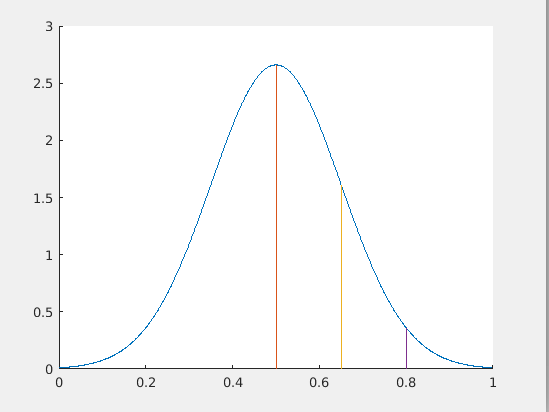
\includegraphics[scale=1]{lecture1_fig1.png}
%
%		\newpage
%		\item \textbf{ \LARGE Now let's do an example.  } \\\\
%
%		
%\end{itemize}


	





